\documentclass[tikz,border=7pt]{standalone}
\usepackage[scaled=0.95]{helvet}\renewcommand{\familydefault}{\sfdefault}
\usepackage[europeanresistors,americanvoltages]{circuitikz}
\definecolor{TEJNavy}{HTML}{1E2B55}
\begin{document}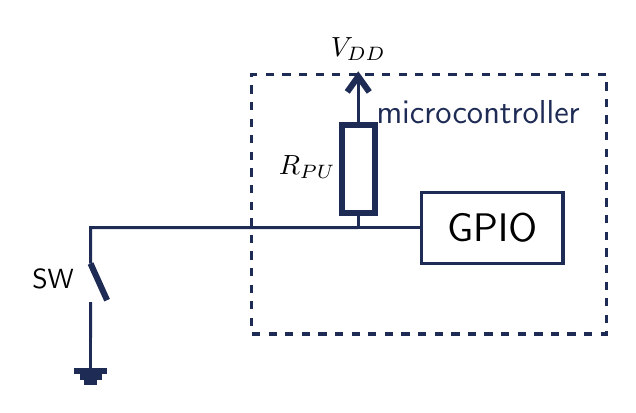
\begin{tikzpicture}[line width=1.1pt,draw=TEJNavy]
\node[draw=TEJNavy,dashed,minimum width=4.5cm,minimum height=3.3cm] (mcu) at (5.7,2.1) {};
\node[font=\large,text=TEJNavy,anchor=north east] at (7.75,3.55) {microcontroller};
\node[draw=TEJNavy,minimum width=1.8cm,minimum height=0.9cm,font=\Large] (pin) at (6.5,1.8) {GPIO};
\draw (4.8,1.8) -- (pin.west);
\draw (4.8,1.8) to[R,l=$R_{PU}$] (4.8,3.3) node[vcc] {$V_{DD}$};
\draw (4.8,1.8) -- (1.4,1.8) to[nos,l_=SW] (1.4,0.4) node[ground] {};
\end{tikzpicture}\end{document}
